% $Id: objectmappingprefs.tex 7846 2009-02-24 13:51:53Z alexandra $
% Local Variables:
% ispell-check-comments: nil
% Local IspellDict: american
% End:
% --------------------------------------------------------
% User documentation
% copyright by BREDEX GmbH 2005
% --------------------------------------------------------
\index{Preferences!Object Mapping}
\index{Object Mapping!Preferences}
\index{Heuristic}
\label{objectprefs}

\begin{itemize}
\item To edit the object mapping preferences, open:\\
\bxmenu{Window}{Preferences}{}\\
and select \bxcaption{Object Mapping} from the left-hand side.
\item In the dialog which appears (see \bxfigref{objectmappingpref}), you can:
\begin{description}
\item[Show number of child nodes:]{activating this option shows the number of items contained in each category. If the \gdomeditor{} is open, you will have to close it and reopen it for the changes to take effect.}
\item[Change the strictness of the object mapping:]{See the next section \bxpref{obprefs} for details.}
\end{description}
\end{itemize}

\begin{figure} [htbp]
\begin{center}
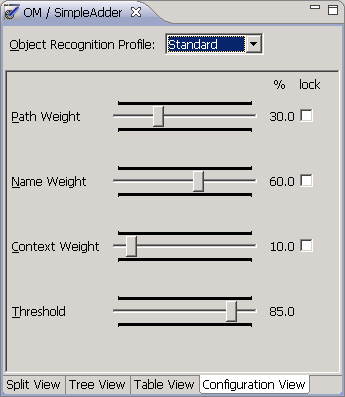
\includegraphics{Tasks/Objectmapping/PS/objectmappingpref} 
\caption{Object Mapping Preferences}
\label{objectmappingpref}
\end{center}
\end{figure}

\subsection{Object mapping preferences: what do the sliders mean?}
\gdhelpid{prefPageObjectMappingContextId}{Object Mapping Preferences}
\label{obprefs}
\begin{itemize}
\item The object mapping in \jb{} is a \bxname{heuristic} process.
\item During test execution, a calculation is made for each component in the \gdaut{} to see how similar it is to the originally mapped component.
\item This calculation is based primarily on the component type -- if you mapped a combo box, only combo boxes will considered.
\item For each component of the same type, the similarity to the original is calculated using three weighted properties:
\begin{description}
\item[Name:]{The name of the component as given by the developer or as generated for the component by \jb{}. }
\item[Path:]{The \bxname{path} to the component is the route followed through the \gdaut{} hierarchy to get to this component. For example, the component is in a dialog box which has two panels.}
\item[Context:]{The \bxname{context} of the component is the other components around it. For example, in the \gdaut{} hierarchy, it is on the same level as a button and a text field.}
 \end{description}
 \item You can see these properties in the object mapping preferences. 
 \item The weighted value for each property is shown on a slider. The sliders can be changed to change the weight of a particular property. See the next section \bxpref{tasksomprefedit} for details.
 \item There are also two other sliders in the object mapping preferences:
 

\textbf{Generated Names Penalty}
\begin{itemize}
\item If the developer did not provide names for objects in the source code, \jb{} generates a name for this component when it is mapped.
\item  With this slider, you can specify a penalty for the name weight property when the names were generated by \jb{}. 
\item In this way, you can have a different name weight calculation depending on whether the name was given or generated.
\bxtipp{The default value for the Generated Names Penalty is 0. You should leave it at this value \emph{if the developers did not provide names for objects in the source code}.}
%%\item  Although the Name Weight itself still counts towards e.g. 60\% of the calculation, a penalty on the value for a generated name will result in the overall value of the Name Weight being lower.
\end{itemize}

\textbf{Threshold}
\begin{itemize}
\item The weighted results from the four previous sliders provide a percentage value of similarity between the originally mapped component and each component that \jb{} finds during test execution.    
\item This slider allows you to specify a minimum percentage at which a component should be accepted. 
\item Components with a percentage value under this threshold are not considered. 
\item The component with the best value above this level is chosen.
\end{itemize}
\end{itemize}

\subsection{Object mapping preferences: editing the sliders}
\gdhelpid{prefPageObjectMappingContextId}{Object Mapping Preferences}
\label{tasksomprefedit}
\bxtipp{The object mapping preferences are valid for all \gdsuites{}, \gdauts{} and \gdprojects{} for each user.  If you change the preferences for one \gdproject{}, for example, ensure that they are returned to \bxcaption{Standard} for other \gdprojects{} if this is necessary. }


\begin{itemize}
\item The sliders specify how important each property is. The higher the percentage of the slider, the more importantly the property will be weighted in the calculation.
\item There are three standard profiles to choose from the combo box in the object mapping preferences.
\item You can also customize the sliders yourself, by selecting the \bxcaption{customize} option.
\item The profiles are:
\end{itemize}

\begin{enumerate}
\item Standard
\begin{itemize}
\item This is the default profile.
\item It has a high value for \bxname{name weight} and lower values for the \bxname{context} and \bxname{path}.
\item Names generated by \jb{} are penalized by 15\%.
\item The threshold is set at 85\%. Components with calculated values lower than this are not considered. 
\end{itemize}

\item Strict
\begin{itemize}
\item The values for \bxname{name}, \bxname{path} and \bxname{context} are the same as in the standard profile.
\item The generated names penalty is set to 0\%.
\item The threshold is set to 100\%. This means that the selected object must exactly correspond to the originally mapped component. 
\end{itemize}

\item Given Names
\begin{itemize}
\item In this profile, only the component name is considered.
\item A component will only be selected if it has the same name as the originally mapped component. 
\item Component names generated by \jb{} are penalized at 100\%, i.e. they will not pass the threshold.
\item The threshold of 100\% ensures that only the component with the same name will be chosen. 
\item This profile can be used when all components in the \gdaut{} have been given distinct names. 
\end{itemize}

\item Custom
\begin{itemize}
\item This profile allows you to move the sliders yourself.
\item You can check the box on the right-hand side of each slider to lock the slider. This stops it being affected when you move other sliders. 
\end{itemize}

\textbf{Name Weight}
\begin{itemize}
\item Increasing the \bxname{name weight} means that the name of the component will be more important in the calculation. 
\item This is good when you know that most or all of the components have been given distinct names by the developers. 
\item A given name is the property most unlikely to change from version to version of the \gdaut{}. 
\end{itemize}
\textbf{Path Weight}
\begin{itemize}
\item Increasing the \bxname{path weight} means that the path through the underlying structure of the GUI will be more important in the calculation.
\item Changes in the GUI may often include a change in the path, so it is a good idea to not place too much importance on this property. 
\item However, unless you are sure that all the names in the \gdaut are distinct, it should not be completely ignored. 
\end{itemize}
\textbf{Context Weight}
\begin{itemize}
\item The \bxname{context} of a component (which other components are ''near'' it) is also likely to change. 
\end{itemize}
\textbf{Generated Names Penalty}
\begin{itemize}
 \item You can change the \bxname{generated names penalty} to increase or decrease the penalty to the calculation if the component name was generated by \jb{}. 
 \item Unlike component names given by developers, component names generated by \jb{} are subject to change. 
 \item If you have placed a large importance on names, it is a good idea to include a penalty for generated names if the names in the \gdaut{} are not all distinct. 
\end{itemize}
\textbf{Threshold}
\begin{itemize}
 \item Increasing the \bxcaption{threshold} increases the overall strictness of the selection. If you set the threshold to 100\%, only components which are exactly the same will be selected. 
\end{itemize}
\end{enumerate}

\bxwarn{Take care when manually customizing the object mapping settings. You may have test execution problems if you have set the values too strictly, or not strictly enough.}
